%----------------------------------------------------------------------------------------
%    PACKAGES AND THEMES
%----------------------------------------------------------------------------------------

\documentclass[aspectratio=169,xcolor=dvipsnames]{beamer}
\usetheme{SimpleDarkBlue}

\usepackage{hyperref}
\usepackage{graphicx} % Allows including images
\usepackage{booktabs} % Allows the use of \toprule, \midrule and \bottomrule in tables
\usepackage[numbers]{natbib}
\usepackage{amsmath, amssymb, amsthm}
\usepackage{microtype}
\usepackage{mathtools}
\usepackage{fontspec}
\usepackage{unicode-math}
\usepackage{tikz}
\usetikzlibrary{arrows.meta, positioning, shapes.geometric}

\graphicspath{{./images/}}

\setbeamertemplate{navigation symbols}{}
\setbeamertemplate{footline}{%
	\leavevmode%
	\begin{beamercolorbox}[wd=\paperwidth,ht=3ex,dp=1ex,center]{footlinecolor}%
		\usebeamerfont{footline}%
		\insertframenumber{} / \inserttotalframenumber\hspace{2em}%
		\insertsection\hspace{2em}%
		\textcopyright\ 2025 Radu Briciu
	\end{beamercolorbox}%
}

\definecolor{customDarkBlue}{RGB}{13, 38, 89}
\setbeamercolor{footlinecolor}{bg=customDarkBlue, fg=white}
\makeatletter
\makeatother
%----------------------------------------------------------------------------------------
%    TITLE PAGE
%----------------------------------------------------------------------------------------

\title{\huge \textbf{Neural Networks for Exotic Option Pricing}}

\author{\small Radu Briciu \\ \tiny BSc Finance, PgDip Quantitative Finance}

\institute
{
	
}
\date{\today} % Date, can be changed to a custom date

%----------------------------------------------------------------------------------------
%    PRESENTATION SLIDES
%----------------------------------------------------------------------------------------

\begin{document}

		\begin{frame}
			% Print the title page as the first slide
			\titlepage
		\end{frame}
		
		\begin{frame}{Overview}
			In this session we explore a proposed method for estimating nonlinear stochastic functions in the context of path dependent financial derivatives
			\tableofcontents
		\end{frame}
	
	%------------------------------------------------
	\section{Introduction}
	%------------------------------------------------
	
		\begin{frame}{Issue}
			How can option pricing be accelerated?
			\begin{figure}[h]
				\centering
				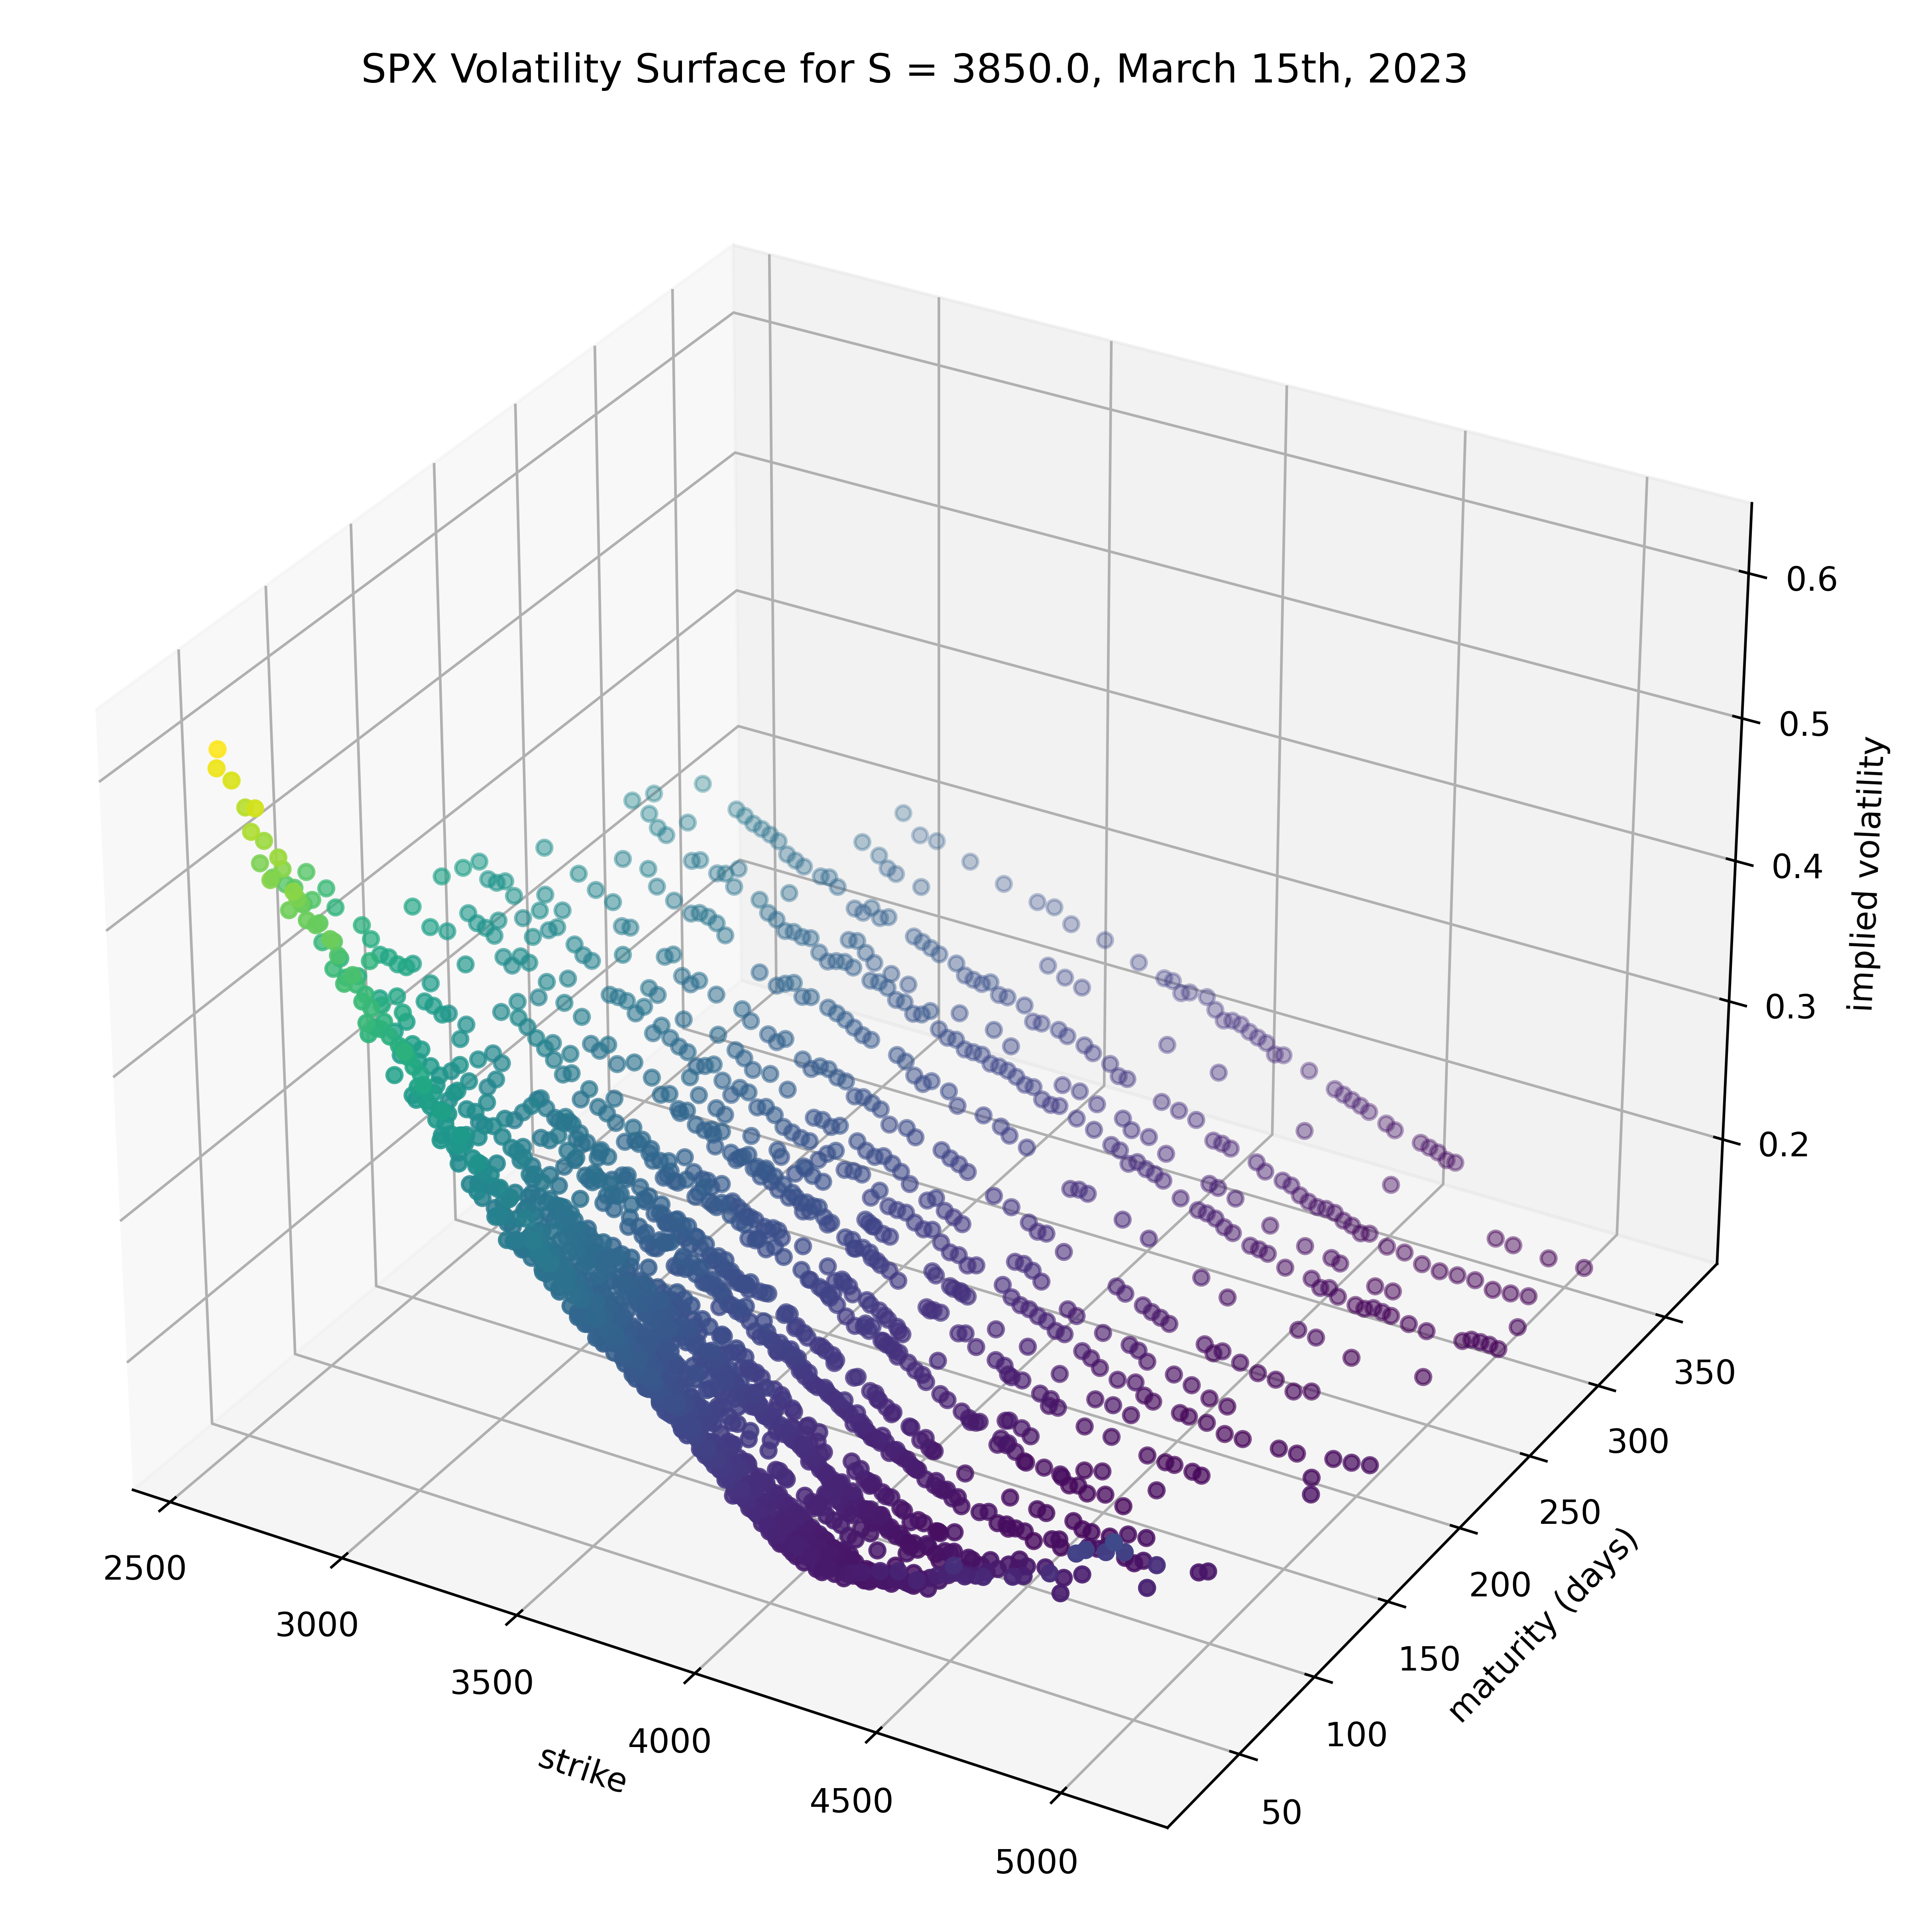
\includegraphics[width=0.4\textwidth]{../../images/surface.png}
			\end{figure}
		\end{frame}
		
%		\begin{frame}{Financial Derivatives}
%			We can begin thinking about the problem by advancing on the illustrious concept of the Myron Black and Fischer Scholes pricing model for European call options.
%			\begin{align}
%				C_{t} &= S_{t} N(d_{1}) - K e^{-r(T-t)} N(d_{2})
%			\end{align} where
%			\begin{align}
%				d_{1} &= \frac{\ln(\frac{S}{K}) + (r+\frac{\sigma^{2}}{2})(T-t)}{\sigma\sqrt{T-t}} \; \; \text{and} \\
%				d_{2} &= d_{1} - \sigma \sqrt{T-t}
%			\end{align}
%		\end{frame}
%		
%		\begin{frame}{Financial Derivatives}
%			Problems with the classical Black-Scholes model (as presented):
%			\begin{enumerate}
%				\item{Constant volatility}
%				\item{Arbitrage free}
%				\item{Instantaneous returns}
%				\item{No dividends}
%				\item{Cannot price complex financial derivatives}
%			\end{enumerate}
%		\end{frame}
		
	%------------------------------------------------
	\section{Pricing Model}
	%------------------------------------------------
	
		\begin{frame}{The Heston (1993) Model}
			\begin{enumerate}
				\item Geometric Brownian Motion
				\item Arbitrary correlation between asset volatility and return
			\end{enumerate}
			\begin{align}
				dS_t &= \left( r - \frac{v_t}{2} \right) dt + \sqrt{v_t} \left( \rho dW_t + \sqrt{1 - \rho^2} dB_t \right) \label{eq:hdXt} \\
				dv_t &= \kappa (\theta - v_t) dt + \eta \sqrt{v_t} dW_t \hspace{1.8cm} \label{eq:hdvt}
			\end{align}
			\begin{enumerate}
				\item $v_0$ represents the initial variance,
				\item $\theta$ is the long-run variance,
				\item $\rho$ is the correlation between the log-price process and its volatility,
				\item $\kappa$ is the mean reversion of the variance to $\theta$,
				\item $\eta$ is the volatility of the variance process, and 
				\item $B_{t}$, $W_{t}$ are continuous random walks.
			\end{enumerate}
		\end{frame}
	
	\section{Exotic Payoff Specifications}
	
		\begin{frame}{Application -- Asian Options}
		Calibration of the Heston (1993) model permits usage of more sophisticated pricing algorithms in determining a correct asset price. We are able to leverage path-dependent dynamics of the underlying price to create more sophisticated financial derivative products. One such example is the \textit{Asian} option:
			\begin{align}
				\label{eq:asianPayoff}
				C^{\text{Asian}}_t &= e^{-r(T-t)} \times \frac{1}{m} \sum_{i=1}^{m} (S_{T}^{\text{avg}} - K)^{+}
			\end{align}
			where $S_{T}^{\text{avg}}$ is the average price of the underlying spot price
		\end{frame}
		
		\begin{frame}{Application -- Asian Options}
			\begin{align}
				C^{\text{Asian}} = F_{t}(S_0, \kappa, \theta, \rho, \eta, v_{0}, r, g, K, n, P, D^{\text{call/put}}, D^{\text{Arithmetic/Geometric}}) \label{eq:Casian}
			\end{align}
			where the price of an Asian option is a function of:
			\begin{enumerate}
				\small
				\item the underlying security price $S$~\eqref{eq:hdXt}, 
				\item the mean reversion speed $\kappa$ of the variance process to $\theta$~\eqref{eq:hdvt}, 
				\item the long-run mean of the variance process $\theta$~\eqref{eq:hdvt}, 
				\item the correlation $\rho$ between the variance process $v_t$ and the underlying price process $X_t$~\eqref{eq:hdXt}, 
				\item the volatility of the variance process $\eta$~\eqref{eq:hdvt}, 
				\item the initial volatility $v_{0}$~\eqref{eq:hdvt}, 
				\item the risk-free rate $r$, 
				\item the dividend rate $g$, 
				\item the strike price $K$, 
				\item the number of fixing dates $n$, 
				\item the number of past fixings$P$ which for our current purposes is always equal to zero, 
				\item a logical operator $D^{\text{call/put}}$ to denote the underlying European option payoff function, and
				\item a logical operator $D^{\text{Arithmetic/Geometric}}$ denoting the averaging type~\eqref{eq:asianPayoff},
			\end{enumerate}
		\end{frame}
		
		\begin{frame}{Application}
		An even less trivial application could be pricing of barrier options.
			\begin{align}
				\begin{aligned}
					C^{\text{payoff}}_{\text{UpIn}} &= \mathbb{1}_{\{ S_t > B \,\forall\, t \}} \times (S_{T}-K)^{+}, \\
					C^{\text{payoff}}_{\text{UpOut}} &= \mathbb{1}_{\{ S_t < B \,\forall\, t \}} \times (S_{T}-K)^{+}, \\
					C^{\text{payoff}}_{\text{DownIn}} &= \mathbb{1}_{\{ S_t < B \,\forall\, t \}} \times (S_{T}-K)^{+}, \: \text{and} \\
					C^{\text{payoff}}_{\text{DownOut}} &= \mathbb{1}_{\{ S_t > B \,\forall\, t \}} \times (S_{T}-K)^{+}
				\end{aligned}
				\label{eq:BarrierPayoffs}
			\end{align}
		\end{frame}
		
		\begin{frame}{Applications}
			\begin{align}
				C^{\text{Barrier}} = F_{t}(S_0, \kappa, \theta, \rho, \eta, v_{0}, r, g, K, B, R, D^{\text{call/put}}, D^{\text{DownIn/DownOut/UpIn/UpOut}}) \label{eq:Cbarrier}
			\end{align}
			\vfill
			Where the price of one Barrier option contract $C^{\text{Barrier}}$ is a function of
			\begin{enumerate}
				\small
				\item the underlying security price $S$~\eqref{eq:hdXt}, 
				\item the mean reversion speed $\kappa$ of the variance process to $\theta$~\eqref{eq:hdvt}, 
				\item the long-run mean of the variance process $\theta$~\eqref{eq:hdvt}, 
				\item the correlation $\rho$ between the variance process $v_t$ and the underlying price process $X_t$~\eqref{eq:hdXt}, 
				\item the volatility of the variance process $\eta$~\eqref{eq:hdvt}, 
				\item the initial volatility $v_{0}$~\eqref{eq:hdvt}, 
				\item the risk-free rate $r$, 
				\item the dividend rate $g$, 
				\item the strike price $K$, 
				\item the barrier level $B$, 
				\item the rebate $R$, 
				\item a logical operator $D^{\text{call/put}}$ to denote the underlying European option payoff function, and
				\item a logical operator $D^{\text{DownIn/DownOut/UpIn/UpOut}}$ denoting the barrier contract type~\eqref{eq:BarrierPayoffs},
			\end{enumerate}
		\end{frame}
	
	\section{Implementation}
	
		\begin{frame}{Model Specification}
			\begin{center}
				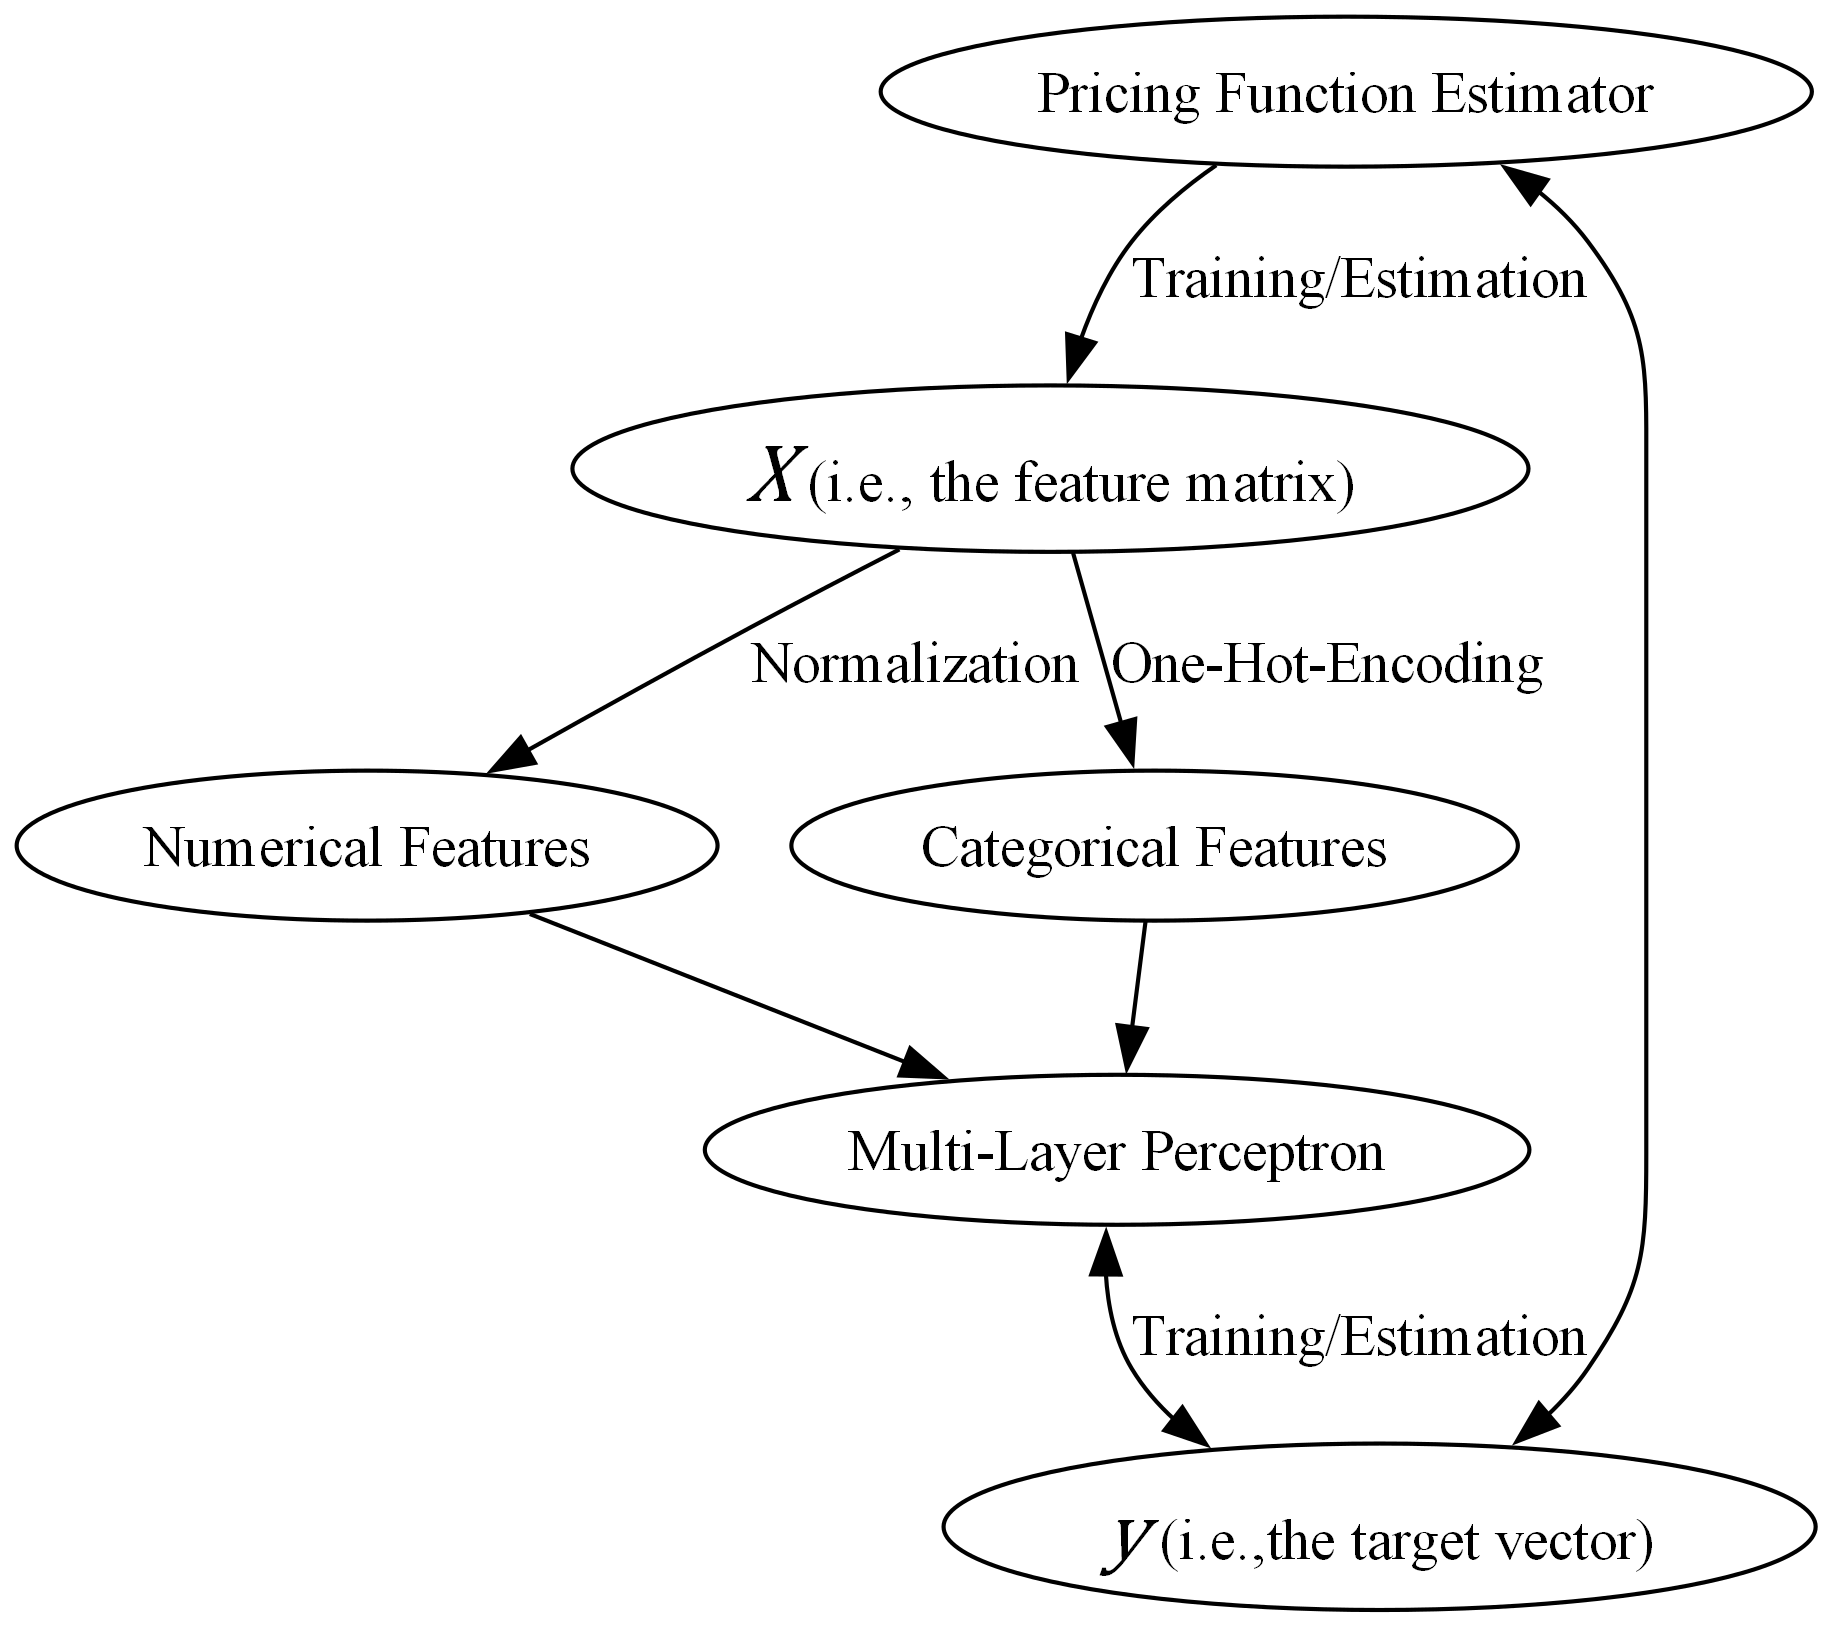
\includegraphics[width=0.5\linewidth]{../../images/MLP.png}
			\end{center}
		\end{frame}
	
		\begin{frame}{Model Specification}
			\resizebox{\textwidth}{!}{%
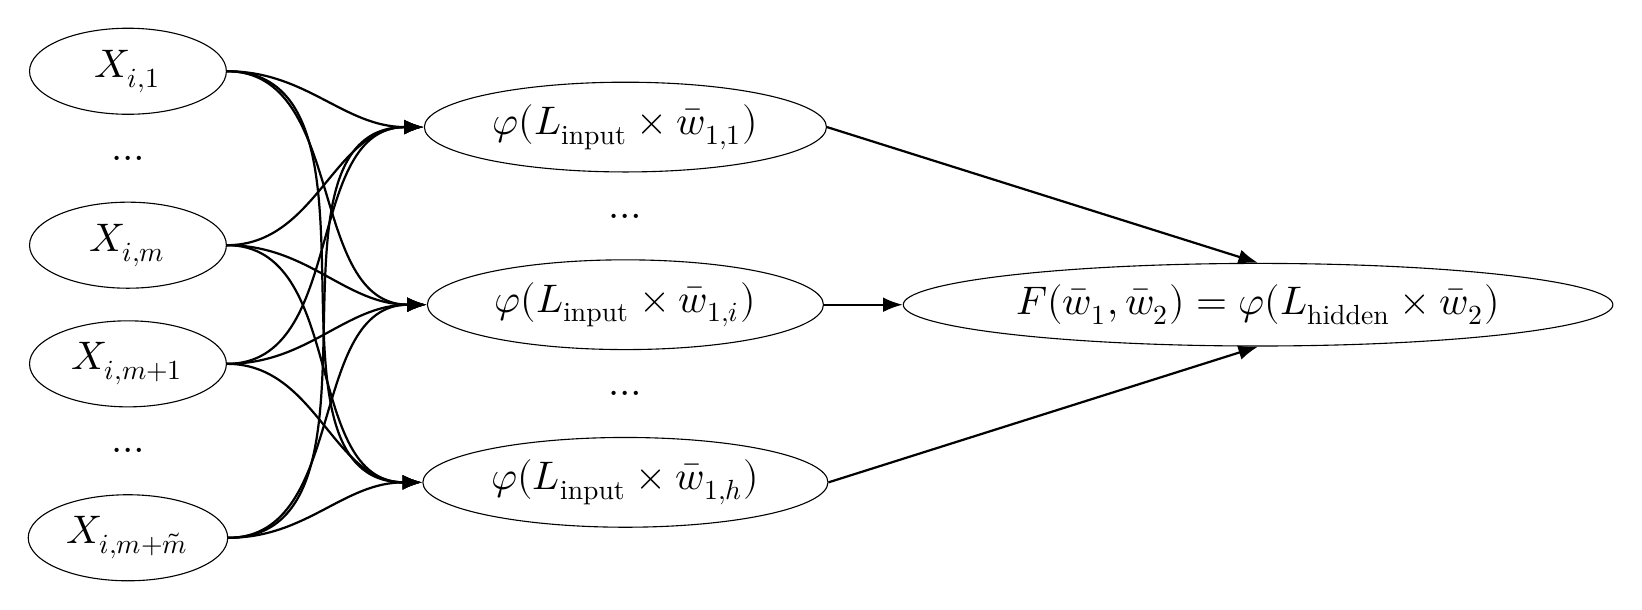
\begin{tikzpicture}[
	every node/.style={font=\Large},
	input/.style={draw, ellipse, minimum width=2.2cm, align=center},
	hidden/.style={draw, ellipse, minimum width=4.5cm, align=center},
	output/.style={draw, ellipse, minimum width=7.5cm, align=center},
	arrow/.style={-{Latex[length=2.5mm]}, thick}
	]
	
	% Input layer (spread vertically)
	\node[input,ellipse,minimum width=2.5cm] (x1) {$X_{i,1}$};
	\node (dots1) [below=0.4cm of x1] {$\hdots$};
	\node[input,ellipse,minimum width=2.5cm] (xm) [below=0.4cm of dots1] {$X_{i,m}$};
	\node[input,ellipse,minimum width=2.5cm] (x1p) [below=0.4cm of xm] {$X_{i,m+1}$};
	\node (dots2) [below=0.4cm of x1p] {$\hdots$};
	\node[input,ellipse,minimum width=2.5cm] (xt) [below=0.4cm of dots2] {$X_{i,m+\tilde{m}}$};
	
	% Hidden layer (centered horizontally and vertically)
	\node[hidden, right=2.5cm of xm, yshift=1.5cm] (h1) {$\varphi(L_{\text{input}} \times \bar{w}_{1,1})$};
	\node (hdots1) [below=0.4cm of h1] {$\hdots$};
	\node[hidden, below=0.4cm of hdots1] (hi) {$\varphi(L_{\text{input}} \times \bar{w}_{1,i})$};
	\node (hdots2) [below=0.4cm of hi] {$\hdots$};
	\node[hidden, below=0.4cm of hdots2] (hh) {$\varphi(L_{\text{input}} \times \bar{w}_{1,h})$};
	
	% Output layer (centered vertically relative to hidden layer)
	\node[output, right=1cm of hi] (out) 
	{$F(\bar{w}_{1},\bar{w}_{2}) = \varphi(L_{\text{hidden}} \times \bar{w}_{2})$};
	
	% Connections (curved)
	\foreach \i in {x1, xm, x1p, xt} {
		\draw[arrow] (\i.east) to[out=0,in=180] (h1.west);
		\draw[arrow] (\i.east) to[out=0,in=180] (hi.west);
		\draw[arrow] (\i.east) to[out=0,in=180] (hh.west);
	}
	
	\draw[arrow] (h1.east) -- (out.north);
	\draw[arrow] (hi.east) -- (out.west);
	\draw[arrow] (hh.east) -- (out.south);
	
\end{tikzpicture}
}
			\[ \min_{w_{1}, w_{2}} \, \frac{1}{N} \sum_{i=1}^{N} \left(F_{t}(w_{1}, w_{2}) - y_{t}\right)^{2} \]
%			\begin{center}
%				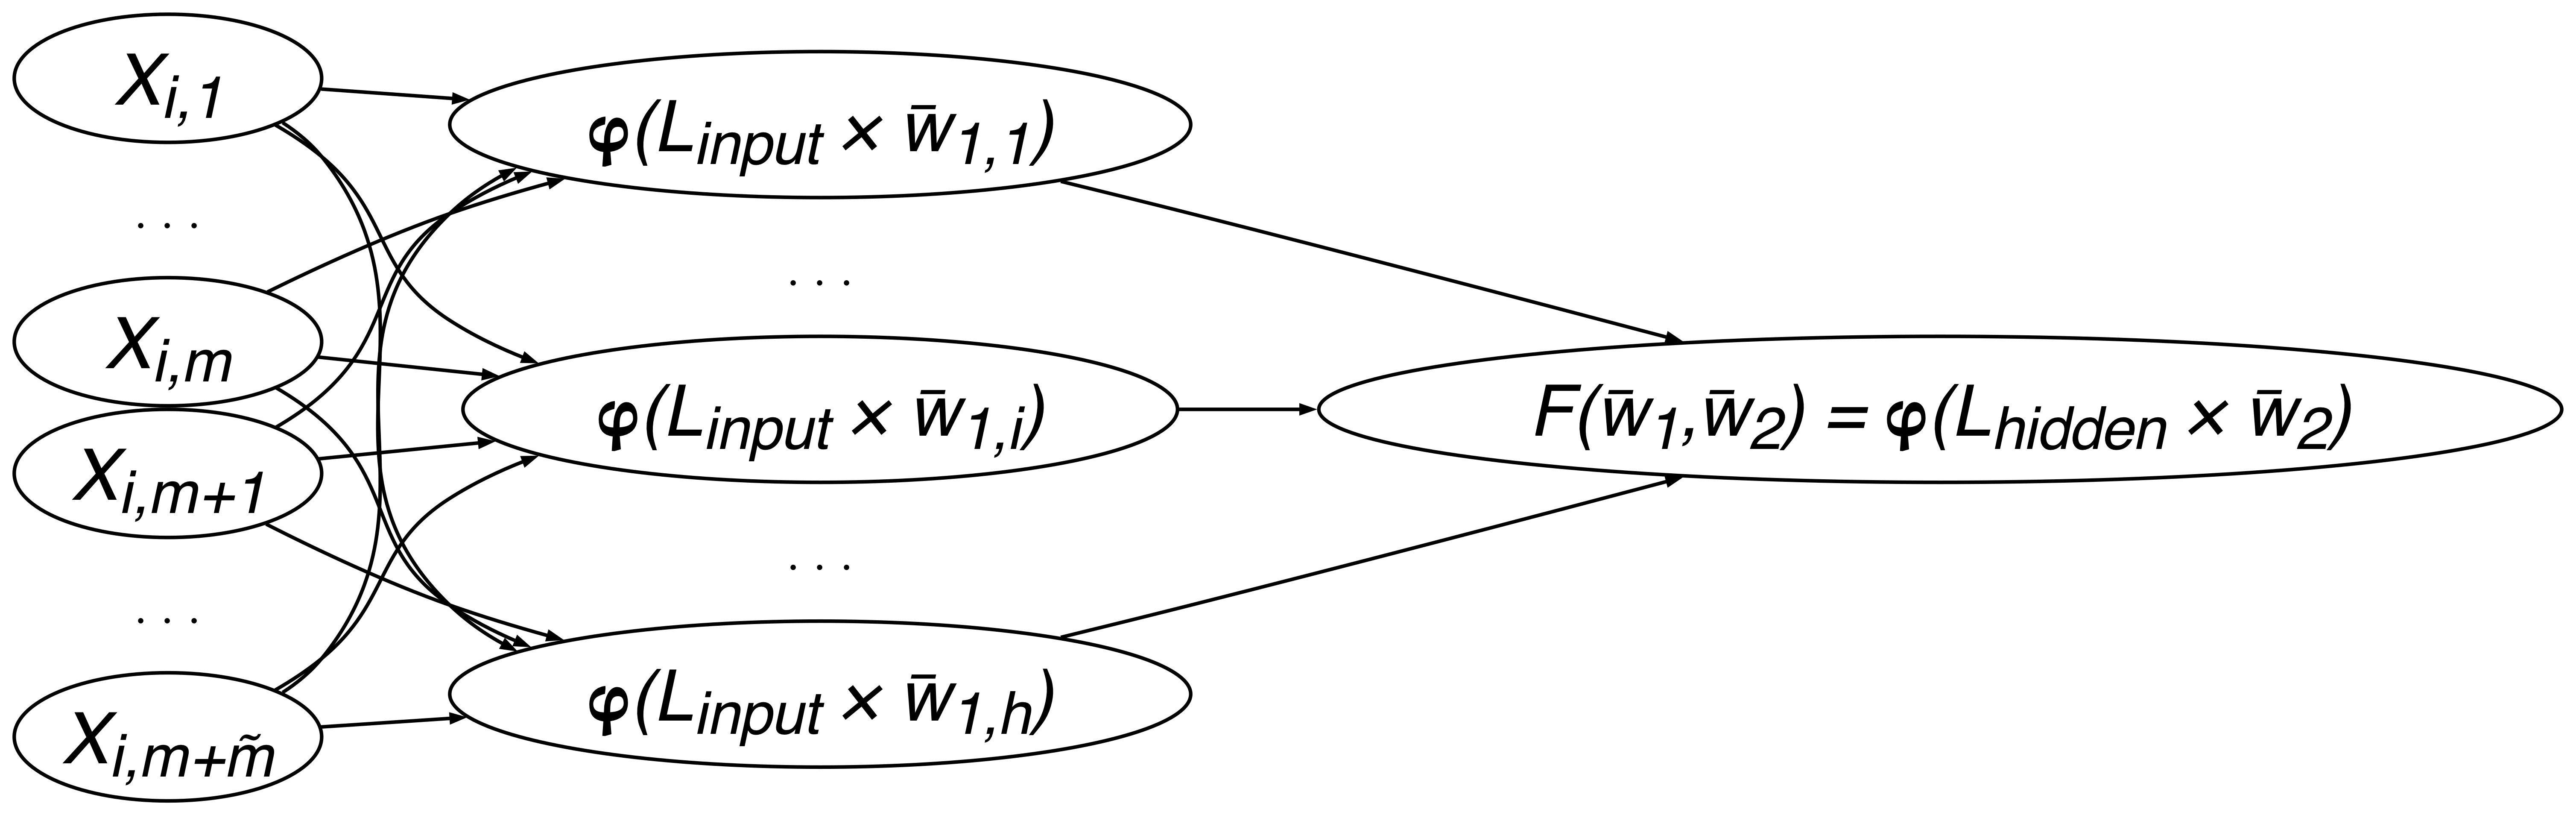
\includegraphics[width=\linewidth]{../manuscript/images/elip.png}
%			\end{center}
		\end{frame}
		
	\section{Challenges}
	
		\begin{frame}{Implementation Hurdles}
		\begin{center}
			\huge \textbf{Implementation Hurdles}
		\end{center}
		\vspace{5em}
		\begin{enumerate}
			\item High initialisation costs
			\item Continuous maintenance
			\item Abnormal distributions
			\item Idiosyncratic risk
		\end{enumerate}
		\end{frame}
		
	\section{Appendix}
		\begin{frame}{References}
			\begin{thebibliography}{9}
				
				\bibitem{boomelage2025a} boomelage (2025). \emph{Machine Learning Option Pricing}. \\
				\url{https://github.com/boomelage/machine-learning-option-pricing}
				
				\bibitem{boomelage2024a} boomelage (2024). \emph{Option Generator}. \\
				\url{https://github.com/boomelage/OptionGenerator}
				
				\bibitem{boomelage2024b} boomelage (2024). \emph{quantlib pricers}. \\
				\url{https://github.com/boomelage/quantlib_pricers}
				
				\bibitem{boomelage2024c} boomelage (2024). \emph{sklearn convencience wrappers ``convsklearn''}. \\ 
				\url{https://github.com/boomelage/convsklearn}
				
				\bibitem{briciu2025} Briciu, Radu (2025). \emph{Neural Networks for Exotic Option Pricing}. 
				\url{https://doi.org/10.2139/ssrn.5104328}
				
				\bibitem{quantlib} \emph{QuantLib Pricing Library} \\ 
				\url{https://www.quantlib.org}
				
			\end{thebibliography}
		\end{frame}
		
		
		\begin{frame}
			\centering
			\Huge{\textbf{The End}}
		\end{frame}
	
\end{document}